\documentclass[12pt,aas_macros,twoside]{report}
\usepackage[utf8]{inputenc}
\usepackage[english]{babel}
\usepackage{csquotes}
\usepackage{amsmath}
\usepackage{amsfonts}
\usepackage{amssymb}
\usepackage{amsmath}
\usepackage{mathpazo}
\usepackage{graphicx}
\usepackage{afterpage}
\usepackage{fancyhdr}
\usepackage{setspace}
\usepackage{indentfirst}
\pagestyle{fancy}
\fancyhead[RO]{}
\fancyhead[LE]{}

% \setlength{\parindent}{6em}
\onehalfspace
% \renewcommand{\baselinestretch}{1.4}
% \renewcommand{\arraystretch}{1.5}

\usepackage[caption=false]{subfig}
% \newcommand\mynotes[1]{\textcolor{red}{#1}}
\usepackage[draft]{todonotes}

\usepackage{comment}

%\usepackage[round]{natbib}
\usepackage[a4paper,width=150mm,top=25mm,bottom=25mm]{geometry}
\graphicspath{ {images/} }

\usepackage{aas_macros}
\usepackage[backend=biber,style=authoryear]{biblatex}
\addbibresource{references.bib}


\begin{document}
\begin{titlepage}
    \begin{center}
        
        \vspace*{5cm}
        {\fontsize{50}{60}\selectfont \textbf{Title Here}}
        
        
        \vspace{3cm}
        
        \Huge
        \textbf{Andrei Cuceu}
        
        % \huge
        % Astrophysics MSci
        
        \vspace{1cm}
        
        \huge
        \textbf{Supervisor: Dr.\ Andrew Pontzen}
        
        \vspace{7cm}
        
        \huge
        University College London
        
        \vspace{0.5cm}
        \huge
        \today
        
    \end{center}
\end{titlepage}



\chapter*{\Huge Abstract}

\cite{Eisenstein_BAOpeak_reconstruction}

\tableofcontents

\newpage
\chapter{Introduction}
\Huge
SOME STUFF HERE

\newpage
\chapter{The Growth of Structure}
% \Huge

\todo[inline]{Introduce cosmic variance somewhere}

\section{Perturbation Theory}

\subsection{Overview}

The evolution of primordial perturbations into the structure we detect today is studied analytically using Perturbation Theory (PT). This field can be divided, according to the frame used to study the Universe, into Eulerian PT and Lagrangian PT (LPT). In the Eulerian frame the evolution of the spatial distribution of particles is studied (\cite{Bernardeau_PT}). On the other hand, in the Lagrangian frame, particles are tracked and their evolution with time is studied.

The Eulerian frame has been so widely used to study the growth of perturbations, that we refer to it as Standard Perturbation Theory (e.g. \cite{1983MNRAS.203..345V}, \cite{peebles1980large}). The most popular approach is to consider an irrotational fluid characterized by its overdensity and peculiar velocity distributions (\cite{Carlson_perturbation_theory}). However, this method suffers from divergences at large wavenumbers (on small scales). This lead to a number of extensions meant to bring it under control (\cite{2006PhRvD..73f3519C},~\cite{2008PhRvD..77b3533C}). 

Lagrangian Perturbation Theory has been well developed in the 1990s (\cite{1992MNRAS.254..729B},~\cite{1993MNRAS.264..375B},~\cite{1994MNRAS.267..811B}). However, it has received less attention partly because the method breaks down after shell-crossing (\cite{Carlson_perturbation_theory}). This event will be discussed further in Section 2.2. Recently it has been demonstrated that LPT correctly reproduces the SPT power spectrum, but also even it's linear first order approximation correctly predicts the decay of the correlation between the final (non-linear) and the initial fields (\cite{2008PhRvD..77f3530M},~\cite{2008PhRvD..78h3519M}). As this correlation is the main tool used in this project, our main focus is on the Lagrangian Frame. 

\subsection{The Zel'dovich Approximation}

The central object of Lagrangian Perturbation Theory is the displacement field $\Psi(\textbf{q})$ which maps the initial particle positions expressed by the Lagrangian coordinate $\textbf{q}$ to the final Eulerian particle positions $\textbf{x}$ (\cite{Bernardeau_PT}):
\begin{equation}
     \textbf{x}(t) = \textbf{q} + \Psi(\textbf{q}, t)
\end{equation}

The first order approximation to this equation leads to a separation of variables $\textbf{q}$ and $t$ (\cite{1993sfu..book.....P}). After also adding the expanding background we obtain:
\begin{equation}
    \textbf{r}(t) = a(t) \textbf{x}(t) = a(t) [\textbf{q} + b(t) \textbf{p}(\textbf{q})]
    \label{eq:2.2}
\end{equation}
Where $\textbf{x}(t)$ is now the comoving Eulerian coordinate.

This approximation was first proposed by \cite{1970A&A.....5...84Z} and it now carries his name, as the Zel'dovich Approximation (ZA). It only works for scales much smaller than the horizon, where Newtonian analysis is possible. However, as our purpose is to study the growth of structure on scales smaller than the BAO, this approximation is a very good starting point. 

An important detail is that the ZA (up to a point) works even in the non-linear regime. This regime is defined in terms of the overdensity $\delta$. When $\delta \sim 1$ we enter the non-linear regime. Standard Perturbation Theory generally breaks down at this point. However, by switching to a description in terms of the particle trajectories, we can reach non-linear density contrasts without the particles being perturbed too much (\cite{1993sfu..book.....P}).

On a final note, the ZA is very good at predicting the loss of correlation between the initial and the final density fields (e.g.~\cite{2016PhRvD..93j3519P}). With all these considerations in mind, in this project we will investigate reconstruction methods within the Zel'dovich Approximation.

\section{The non-linear regime}

\subsection{Cosmological simulations}
 However, once we get into the deeply non-linear regime, these methods break down. Instead we rely on large N-body simulations to continue our study of the evolution of structure.

Generally, these simulations are used to help constrain Cosmological theories of the primordial universe or to test perturbation theories. A random initial field with properties based on the CMB and our general understanding of the early universe, is evolved through time until the present. The output of the simulation is then compared to observational data. Simulations like Millennium XXL (\cite{Millennium_XXL}) or Illustris (\cite{Illustris_sim}) gave us an unprecedented insight into structure formation and evolution.

On the other hand, simulations are also used as a laboratory for testing reconstruction methods they give us access to both the initial and the final density fields. We can attempt a reconstruction on the final field and then compare it to the initial field and test how well it worked. 

\subsection{Information loss}


\todo[inline]{Talk about the Linear regime of collapse versus the non-linear regime. Present the difficulty of constructing analytical models of non-linear collapse. Motivate our use of simulations as well as our desire to get back to the linear regime for reconstruction.}

\section{Reconstruction}

This can be understood by thinking about the difference between looking at the large scales versus the small scales. For example, a very large (by scale) primordial underdensity will probably still be an underdensity at late times (as a huge void). However, on small scales, information tends to be destroyed. A small scale primordial underdensity might be caught in the larger bulk flows and collapse in a larger halo. In this case, the information about the small underdensity is lost. \todo{this paragraph could go in chapter 2}


\todo[inline]{Finally link everything with an overview of Reconstruction techniques and how our work fits into the modern context.}

\todo[inline]{Showcase the BAO reconstruction.}

% \begin{figure}
%     \centering
%     %\hspace*{\fill}
%     \subfloat[]{
%       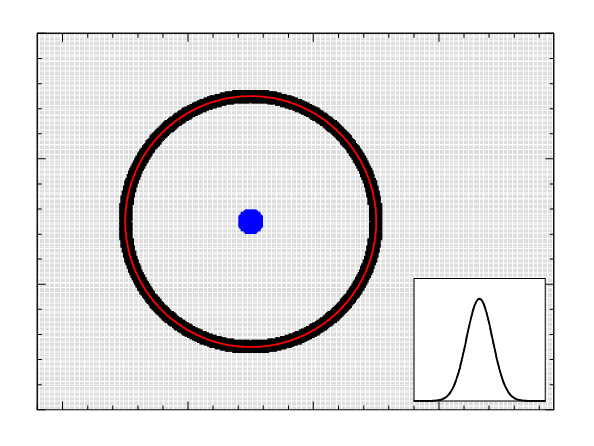
\includegraphics[width=0.45\columnwidth]{images/misc/slice000.png}%
%     }\hfill
%     \subfloat[]{
%       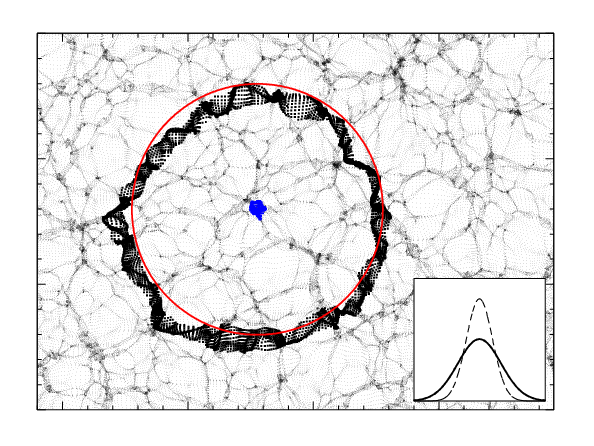
\includegraphics[width=0.45\columnwidth]{images/misc/slice040.png}%
%     }\hfill
%     \subfloat[]{
%       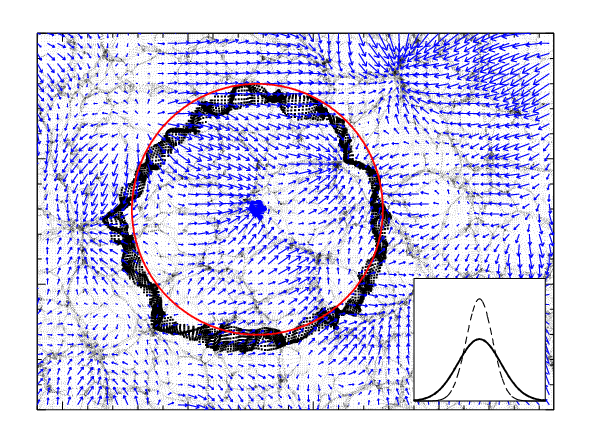
\includegraphics[width=0.45\columnwidth]{images/misc/vector040.png}%
%     }\hfill
%     \subfloat[]{
%       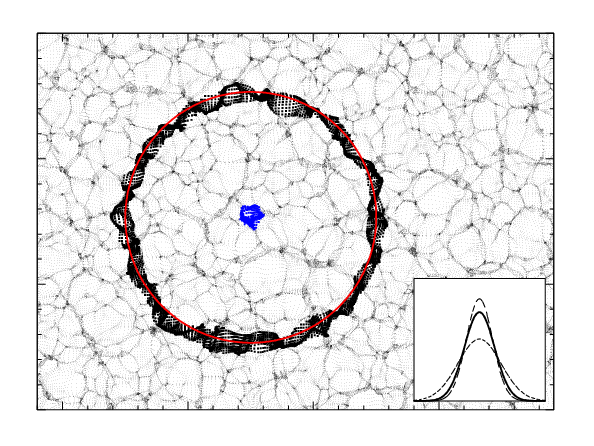
\includegraphics[width=0.45\columnwidth]{images/misc/recon040.png}%
%     }\hfill
    
%     \caption{
%       \setstretch{1.0}
%       \small
%     An illustration taken from~\cite{2012MNRAS.427.2132P}, showing how the acoustic scale is distorted by non-linear effects and then reconstructed. (a) In the early Universe, the density field was very smooth. The acoustic feature is marked with a ring of radius $150Mpc$, and the distance between the centroid (blue point) and the radially distributed black points is represented by a Gaussian. (b) In the late Universe, non-linear effects move the points on the acoustic scale from their original positions (still represented by the red circle). This can be seen as a broadening of the radial distribution (dashed line is the original). The evolution here was modelled using the Zel'dovich approximation. (c) The Lagrangian displacement field (blue arrows) is calculated. The concept behind reconstruction techniques is to estimate the displacement field in order to move the particles back to their original position. The field was smoothed using a Gaussian filter. (d) The particles were moved back along the displacement field, and a clear improvement can be seen. The solid line marks the reconstructed radial distribution, the dashed line represents the primordial distribution, and the dotted line is the late time distribution before reconstruction. In this case the reconstruction is not perfect because of the Gaussian filter, which was used to mimic a real scenario. Note that this was done just for illustration purposes, and actual reconstruction methods are more complex.
%     }
    
% \label{fig:3}
% \end{figure}

% \section{The Matter Power Spectrum}

% As our objective is to reconstruct the final density field and compare it to the initial one, we need a good way of describing the two fields. A widely used method is to look at the Matter Power Spectrum. We first start with the overdensity $\delta$:
% \begin{equation}
%     \delta(\textbf{x}) = \frac{\rho(\textbf{x}) - \overline{\rho}}{\overline{\rho}}
% \end{equation}
% where $\rho(\textbf{x})$ is the density at $\textbf{x}$, and $\overline{\rho}$ is the average density. The spatial average of this overdensity field is not a good characterization as it is equal to 0. Instead we look at its variance, the correlation function:
% \begin{equation}
%     \xi
% \end{equation}

% \newpage
% \chapter{Methods}
% \Huge
SOME STUFF HERE

\newpage
\chapter{The Perfect Reconstruction}
% \Huge

% \todo[inline]{The section names here are just temporary.}
Our first step is to try to understand how much information from the primordial Universe is preserved. We will look at the theoretical limit encountered when trying to reconstruct the final non-linear density field. 

As a field is defined at every point in space, any attempt at representing it with data is inherently imperfect. We would have to measure the density field at every point in the Universe in order to obtain all the information it contains. This fact already implies that no data driven reconstruction will ever succeed at perfectly recovering the primordial density field (unless we manage to make an infinity of measurements).

To show this unavoidable loss of information we performed a `perfect' reconstruction. We call this reconstruction `perfect', as it uses data about the initial positions of all particles (which obviously is not available to observers). However, as we will show in this chapter, not even this perfect reconstruction succeeds at perfectly recovering the primordial matter distribution.

\section{Methods}

% \todo[inline]{Present how we did the perfect reconstruction}

The first step in studying reconstruction is to find a way to test its effectiveness. To do this, we use cosmological N-body simulations. These simulations give us important insights into how structure evolves in the Universe. More importantly for this project, it allows us to compare any reconstructed density field to the real starting density field. We use data from three simulations available to us. The first one is Simulation A presented in~\cite{Pontzen_paired_simulations} (also referred to as Simulation A in this work). The other two simulations are variations of the same initial setup, with smaller size and smaller resolution respectively. The details of all three simulations are presented in Table 1.

\begin{table}[h!]
    \centering
    \begin{tabular}{ |c|c|c|c| } 
        \hline
        Label & Size & Number of Particles & Particle Mass (Solar Masses) \\
        \hline
        Sim A & $(200 Mpc)^3$ & $512^3$ & $6.59 \times 10^9$ \\ 
        \hline
        Sim B & $(200 Mpc)^3$ & $256^3$ & $5.27 \times 10^{10}$ \\ 
        \hline
        Sim C & $(100 Mpc)^3$ & $256^3$ & $6.59 \times 10^9$ \\ 
        \hline
        
    \end{tabular}
    \caption{Details of the three simulations used in this project. They were setup in away that allows us to study the impact of the resolution (Sim A vs Sim B) and size (sim A vs Sim C)}
    \label{table:1}
\end{table}

The simulations only contain dark matter and the cosmological parameters used were the ones recommended by the WMAP 7-year observations (\cite{2011ApJS..192...18K}). These are no longer our best estimates (\cite{2016A&A...594A..13P}), however for our present purposes they are sufficient as we do not compare to observational data. The simulations were evolved from $z=99$ to $z=0$ using the \textsc{P-Gadget-3} code (\cite{2005MNRAS.364.1105S},~\cite{2008MNRAS.391.1685S}). 

The idea behind a perfect reconstruction is to use data about the initial state of the simulation to perform the reconstruction. We have access to multiple snapshots at various redshifts in our simulations, including the initial positions of all particles (at $z = 99$). Therefore, we used this information to reconstruct the density field. We first measured the density field of various snapshots in the redshift interval $z = 0 - 9$. The field was measured at the particle positions instead of being measured on a regular grid. This is because the density field will be moved along with the particles as described in the next section. After that, the particle positions were replaced with their initial positions taken from the initial snapshot at $z = 99$.


\section{From Images to Statistics}

% \todo[inline]{Show some density slices of the results, and talk about the effects that pop up (e.g. the increase in total mass). Show Power Spectra}

\subsection{The Reconstructed Density Field}

As outlined above, the first step is to measure the density field in a snapshot. Each snapshot contains an indexed list with the positions, velocities and masses of all particles in the simulation. In this chapter, only the positions and masses are needed to perform a perfect reconstruction. To perform the first part of this analysis, we used the \textit{pynbody}\footnote{https://github.com/pynbody/pynbody} package (\cite{2013ascl.soft05002P}). 

\begin{figure}
    \centering
    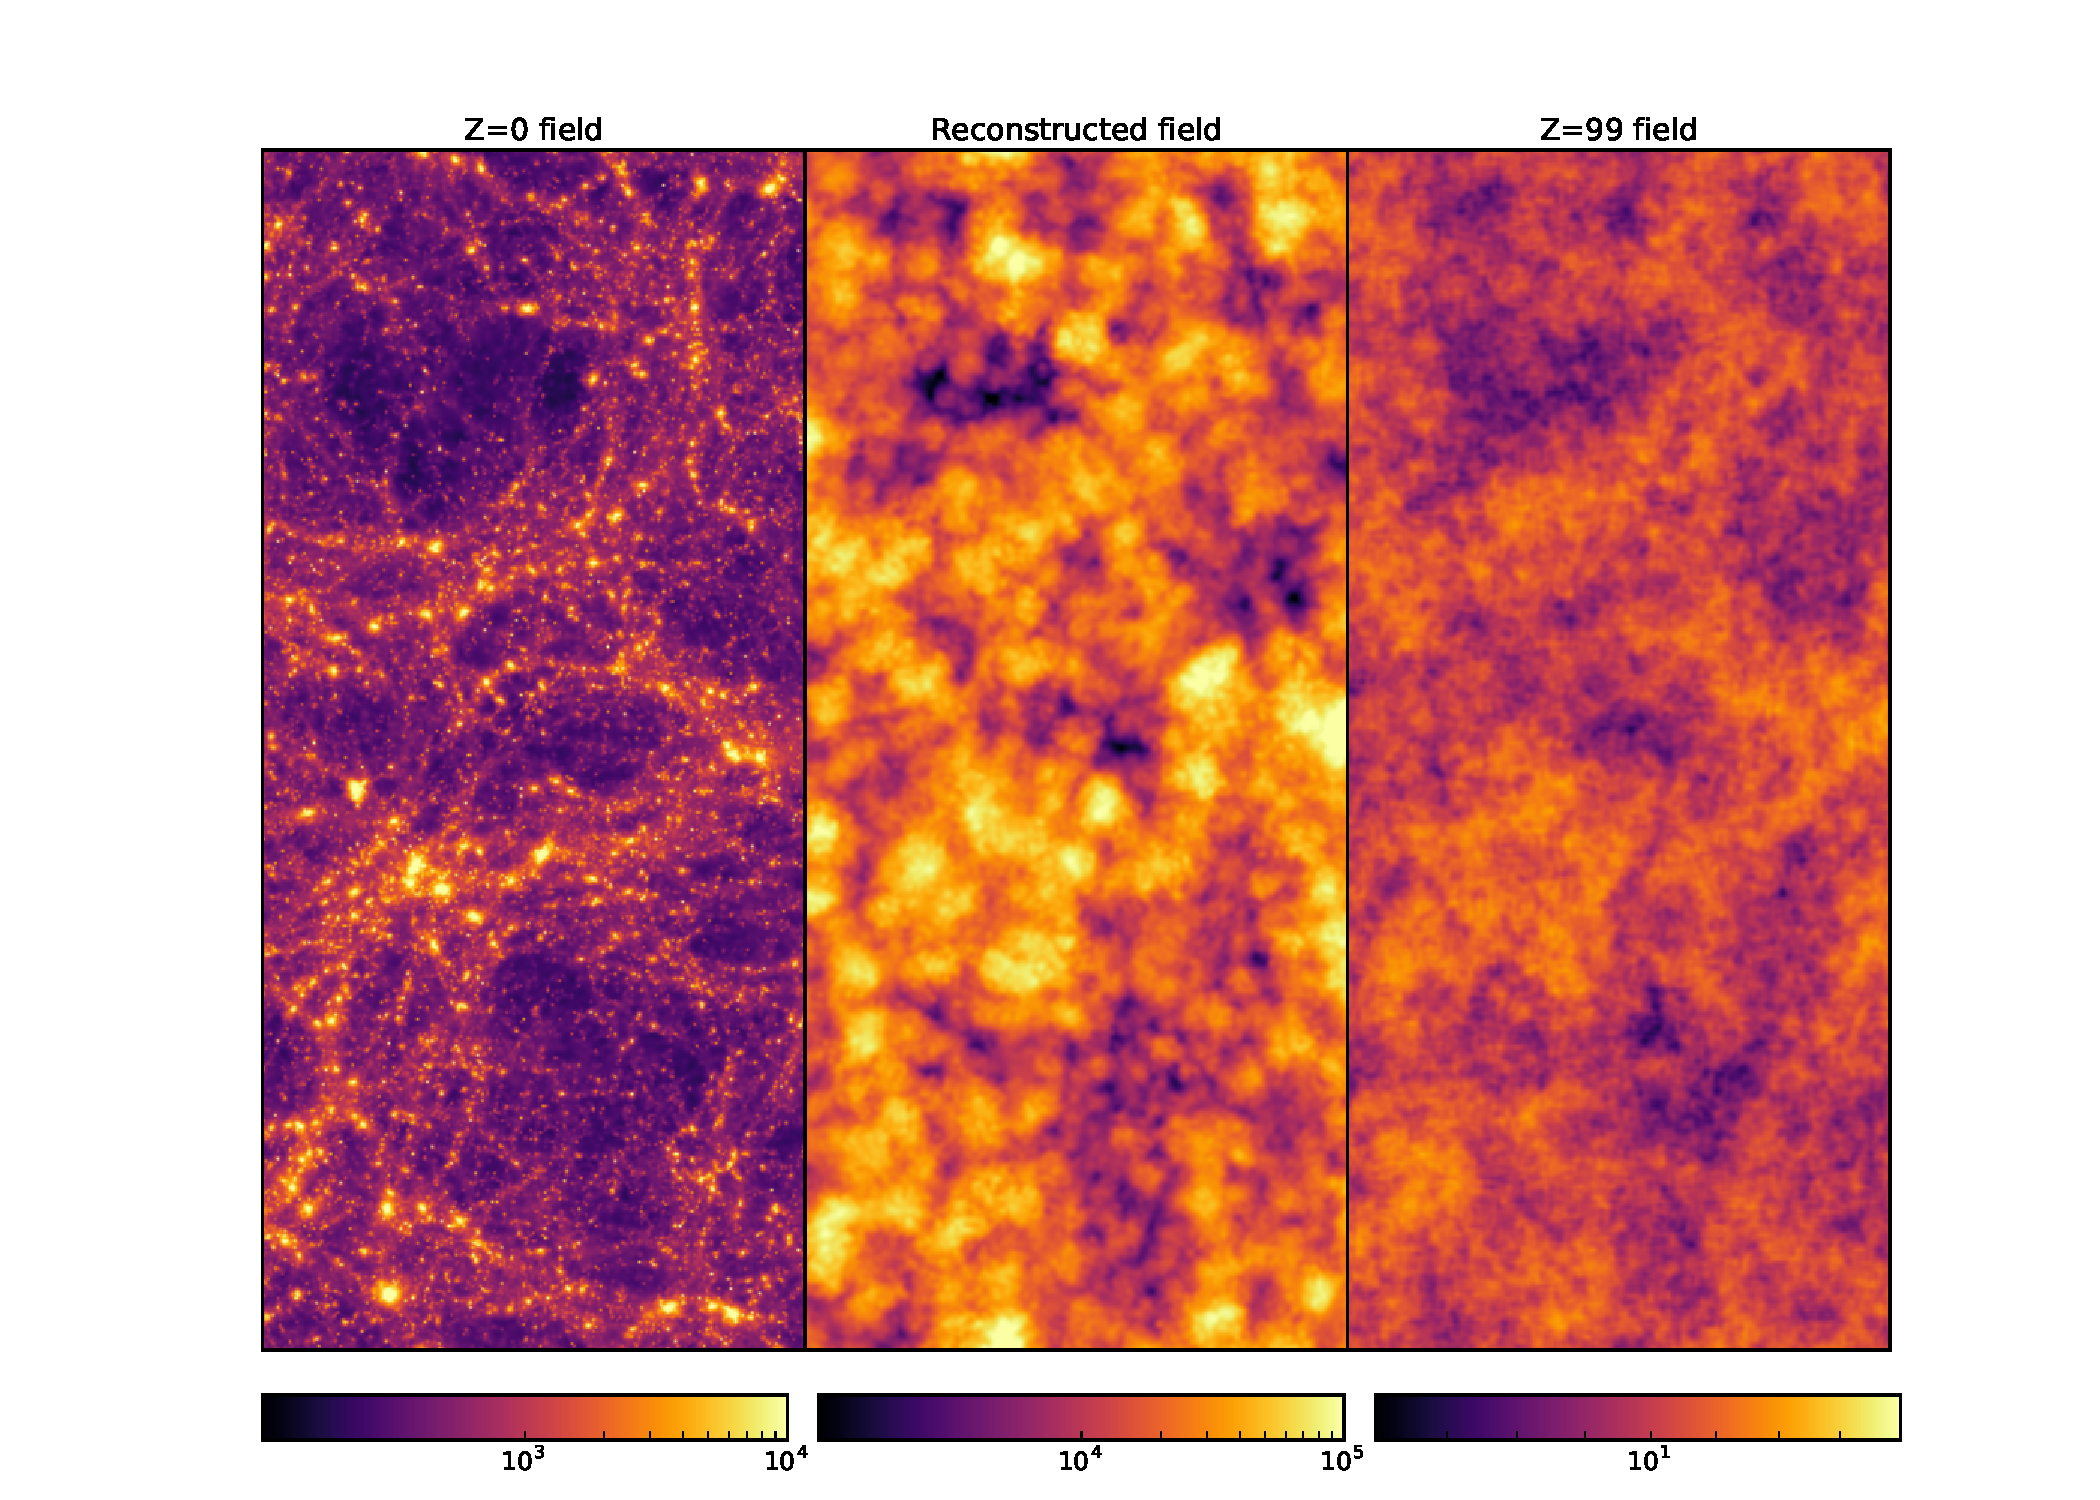
\includegraphics[width=1\columnwidth]{images/densityFields/densityField.pdf}%
    
    \caption{
    Density slice through Simulation C. The left panel shows the final collapsed density field at redshift 0. The right panel shows the initial smooth density field at redshift 99. The centre panel shows the result of the perfect reconstruction applied to the final field. The collapsed filaments are stretched, but the result is not identical to the initial field. This means there is some information that cannot be recovered.
    }
    
    \label{im:1}
\end{figure}

To have a visual understanding of the reconstruction, we first make some images of the density field. We use \textit{pynbody} to import the initial snapshot and the snapshot at $z=0$. The density field at the particle locations in the final snapshot is calculated and assigned as the density field of the initial snapshot. Density slices through this reconstructed field are compared to the initial and final fields in Figure~\ref{im:1}. 

We can already see from this comparison that the reconstruction has not recovered all the information, as it is not identical to the initial filed. However, the reconstruction spreads out the matter from the collapsed filaments onto a more uniform field. This is exactly the opposite of small initial perturbations collapsing into the filaments. In a way we are trying to run gravity in reverse. Also notice the large difference in the values of the density field. The reconstructed field has density values about 3 orders of magnitude larger than the initial field.

% \todo{also talk about the density distribution}

This large difference is an interesting side effect of our method. At late times, most particles tend to be clumped together. Therefore, when measuring the density field at the particle positions, we will mostly get very high values. These values do not change when moving the particles, so the final field will also have very high values, but this time distributed on an almost uniform grid. This results in an apparent increase in the total mass of the simulation. As this increase is just a result of the way we represent the density field, it needs to be accounted for when analysing the results. To conserve the mass of the simulation, we just divide the density field by the ratio of the total final mass to the total initial mass.

\subsection{Correlation with the Initial Field}

In order to get a better understanding of how well this reconstruction worked, we turn to statistics. A good way to represent the reconstruction is to look at the normalized Cross-Spectrum between the initial and the reconstructed field: $$ \frac{P_{IX}(k)}{\sqrt{P_I(k) * P_X(k)}} $$ where $I$ represents the initial field, and $X$ the reconstructed field. The power spectrum is defined as the Fourier transform of the correlation function of the two fields:
\begin{equation}
    P(k) = \int{d^3y e^{i\textbf{k} \cdot \textbf{y}} \xi(y)}
\end{equation} 
and the correlation function of two density fields is given by:
\begin{equation}
    \xi(|\textbf{x}-\textbf{y}|) = \langle \delta_A(\textbf{x})\delta_B(\textbf{y}) \rangle
\end{equation}

We used the \textsc{GenPK} code\footnote{https://github.com/sbird/GenPK.git} (\cite{2017ascl.soft06006B}) to measure auto and cross power-spectra of \textsc{Gadget} outputs. In order to analyse reconstructed fields, we also modified \textsc{GenPK} to read the fields generated by \textit{pynbody}. However, before calculating the power spectrum, we first calculate the logarithm of the density field. This is an extra step in our reconstruction which has the purpose of reducing the density contrast of the reconstructed field. The initial field has a Gaussian distribution of overdensities. As structure evolves, this distribution becomes skewed towards large scales. It also develops a large positive tail as more and more massive halos are created. However, the negative tail of the function is physically limited by zero density. Therefore, we take the logarithm of this function in an attempt to Gaussianize this distribution and bring it closer to the initial one. We will always perform this step in all our reconstructions.

The original normalized cross-spectra between the initial and the final fields (from Sim A) can be seen in Figure~\ref{fig:3.1}. For small wavenumbers $k$ (corresponding to large scales), the correlation is very good (converges to 1: perfect correlation). On the other hand, for large wavenumbers (corresponding to small scales), the two fields are completely decorrelated. 

\begin{figure}
    \centering
    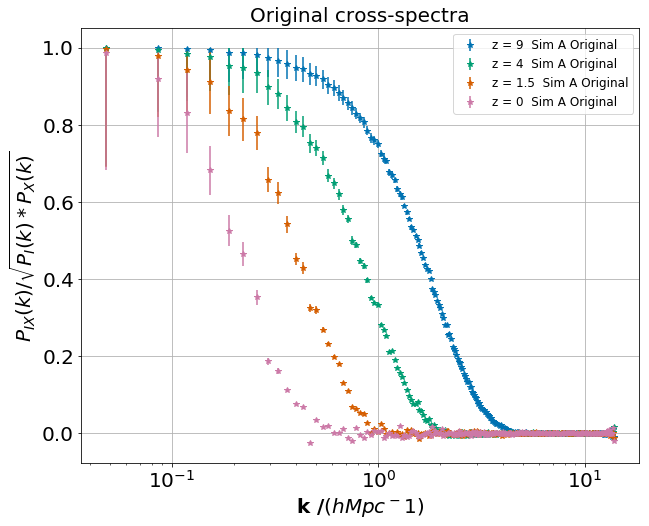
\includegraphics[width=1\columnwidth]{images/perfRecon/orig.png}%
    
    \caption{
    Normalized cross-spectra between the initial and final density fields as a function of scale. At small wavenumbers $k$ (large scales) the two fields are perfectly correlated because the Universe is not affected by gravitational collapse over such scales (they are both uniform). On the other hand, at large $k$ (small scales) they are decorrelated because the initial field is very uniform, while the final field is very non-uniform on such scales (it contains large empty voids, and small and massive halos). The decorrelation scale moves to smaller $k$ as time goes on due to the progressive collapse of larger and larger overdensities.
    }
    
    \label{fig:3.1}
\end{figure}

The small $k$ convergence towards perfect correlation indicates that information is preserved on these scales. Because of this, both the initial and the final density fields tend to be very uniform, which preserves the correlation. However, over small scales information is lost. The results is a large discrepancy between massive collapsed regions and mostly empty voids. This is in stark contrast to the relative uniformity of the initial field, leading to a breakdown in correlation.

Figure~\ref{fig:3.1} also shows the evolution of this correlation with redshift. The wavenumber at which the two fields decorrelate indicates the progress of gravitational collapse at that redshift. This results in the decorrelation scale moving to smaller wavenumbers with the progress of gravitational collapse. The objective of reconstruction methods is to bring this decorrelation scale to larger $k$ (in order to recover information about the initial field).

The errors in Figure~\ref{fig:3.1} come from the measurement of the power spectrum. As we have a limited size box, when we measure the largest scales, we only have access to very few modes. This leads to a large error. The errors were propagated without taking into account the correlations between the power spectra when calculating the normalization. However, as these are definitely correlated, this is just an upper bound of the error. The large scale convergence towards perfect correlation also indicates that the actual errors are much smaller. As such, we will not be including them in the following plots.

\begin{figure}
    \centering
    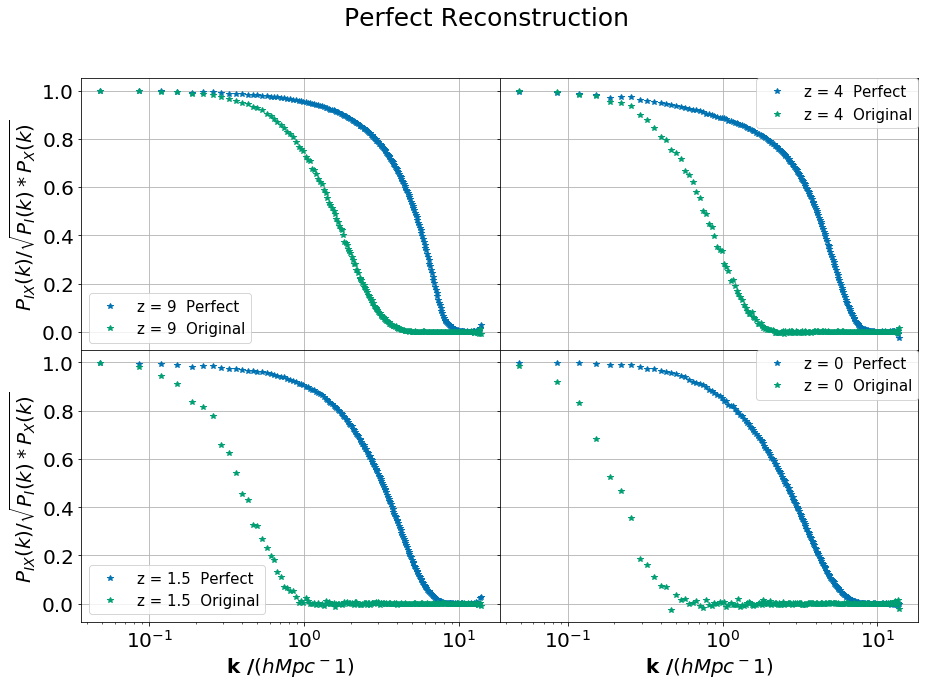
\includegraphics[width=1\columnwidth]{images/perfRecon/perfRecon.png}%
    
    \caption{
    Normalized cross-spectra between the initial and the reconstructed fields compared to the original correlation. A large improvement in the correlation was achieved with the perfect reconstruction. This shows up as a shift of the decorrelation scale towards larger $k$ (smaller scales). However, the perfect reconstruction does not lead to a perfect correlation due to the limiting resolution of our density field measurements. When comparing the reconstruction applied to fields at different redshift, we see a trend towards less information at lower redshift. This shows the progress of information loss between $z=9$ and $z=0$.
    }
    
    \label{fig:3.2}
\end{figure}

\section{Analysis}

The results of the perfect reconstruction can be seen in Figure~\ref{fig:3.2}, where we compare it with the original correlation at different redshifts. The cross-spectra presented show a large improvement in the correlation with the initial field. There is also an increase in the amount of information recovered for lower redshifts. This means redshift does not play a role as large in the perfect reconstruction as it originally did. 

\begin{figure}
    \centering
    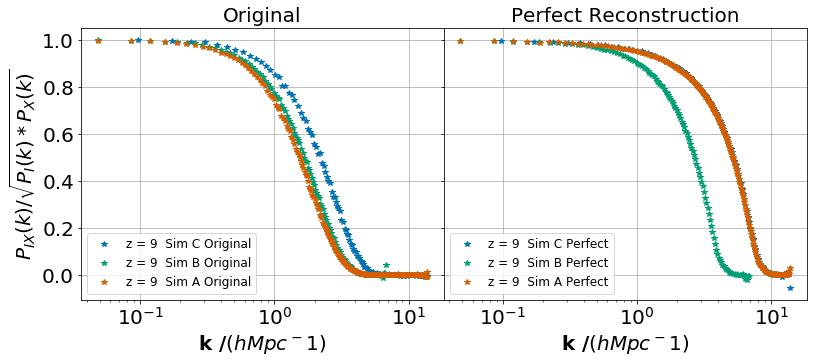
\includegraphics[width=1\columnwidth]{images/perfRecon/simComp.png}%
    
    \caption{
    Normalized cross-spectra across the three simulations. The left plot shows the original correlation between the initial and the final fields, and the right panel shows the correlation with the reconstructed field. For the original correlations, the size of the simulation plays an important role, with the smaller simulation decorrelating on smaller scales. However, after the reconstruction, the size of the simulation does not seem to have any impact (with Sim A being almost identical to Sim C). In this case, the resolution of the simulation is the only factor that matters, with the larger resolution simulations showing a better correlation.
    }
    
    \label{fig:3.3}
\end{figure}
However, in order to understand this perfect reconstruction, we need to look at the key role played by the resolution of the simulation. Figure~\ref{fig:3.3} shows a comparison of the cross-spectra across the three simulations. For the original correlations, the size of the simulation plays a larger role than the resolution. Simulation C (smaller size) shows a smaller scale of decorrelation. Simulations A and B (same size) are very close, with a slight edge for Simulation B (lower resolution). 

A completely different structure can be seen once we perform the perfect reconstruction. Simulation A and C (same resolution) show identical reconstructed correlation, while the reconstruction in Simulation B (lower resolution) does not perform as well. This indicates that resolution plays a decisive role in the perfect reconstruction. The other limiting factor is the starting redshift. As we have seen, more and more information is lost as we go to lower redshift. The right panel in Figure~\ref{fig:3.3} shows the lowest scale that can be reconstructed from $z=9$ depending on the resolution of our simulation.

The reconstructions in Figure~\ref{fig:3.2} demonstrate that a perfect correlation cannot be achieved even in the ideal case of existing knowledge of all the starting particle positions. Therefore, we have shown the limits of reconstruction techniques. However, a large improvement in the correlation can be seen, with the decorrelation scale moving to very small scales (of the order $1 Mpc$). This ideal reconstruction using perfect knowledge of the particle positions serves as a theoretical upper limit to reconstruction techniques. The perfect reconstruction, along with the original correlation, will always be present in the next chapter when we look at realistic reconstructions. This can give us a better understanding to how well our techniques work.




\newpage
\chapter{Towards Realistic Reconstructions}
\Huge

\section{The velocity field}

\section{Getting back to the linear regime}

\section{Results}

\section{Analysis}



\newpage
\chapter{Conclusions}
% \Huge

\section{Information loss and potential recovery}

We studied information loss due to gravitational collapse. Our two main observational probes (CMB and Galaxy surveys) are widely separated by an era from which we have very little information, and which contains such important events as the formation of the first stars and galaxies. It is, therefore, in our interest to find ways of using the data we collect from the Universe today to recover information about the past. Reconstruction techniques have been widely used to recover information on the Baryon Acoustic Peak, but here we look to even smaller scales. Our aim was to test the limits of reconstruction as well as to look at more realistic methods and test their performance.

In Chapter 2, we proved that some information will never be recovered. To show this, a perfect reconstruction was performed. We measured the density field at the particle positions and used the knowledge of the initial particle positions to reconstruct it. Because we do not (and cannot) measure the density field in an infinity of locations, we cannot capture all of its information. This means, no reconstruction is capable of perfectly recovering the primordial density field.

Figure~\ref{fig:3.2} shows the normalized cross spectra of our reconstructed fields with the initial density field (versus the original correlation). Our reconstruction recovers plenty of  intermediate scale information and the two stay correlated to very small scales. However, on these very small scales, they do decorrelate. This information can never be recovered by reconstructing the density field. The plot shows the most amount of information that could ever be recovered from each redshift. In a way, it shows the limit of what we can ever hope to learn about the primordial density field. 

We have also shown that two of the limiting factors in reconstruction are the resolution used and the redshift. Both of these can be improved upon in practice. More and more information is destroyed with the progress of time. By detecting matter further back in time, we increase the amount of information we can recover. On the resolution side, our limitations are the size of galaxies and how many of them we can detect in a certain volume. Galaxies are also biased tracers of matter, therefore galaxy surveys might not be our best option. A very promising future probe is the Square Kilometre Array (SKA:~\cite{dewdney2009square}), as it will push both boundaries at the same time. Its goal is to detect atomic hydrogen before reionisation (using the 21cm emission). As we are looking much further back in time ($z>10$) and directly at the matter distribution, this probe will lead to incredible advancements in our knowledge of the early Universe.


After studying the limits of reconstruction, we turned our attention to more realistic methods in Chapter 3. In particular, we looked at reconstruction methods within the Lagrangian framework. We first start by performing a Zel'dovich reconstruction. Particle velocities are used to calculate a displacement field within the first order approximation of Lagrangian Perturbation Theory (the Zel'dovich Approximation). As before, we calculated the density field at the particle positions and then applied the displacement field to move them back in time. The density field is also carried back in time and reconstructed. We showed that the method works very well when starting at high redshifts ($z=9$). However, when starting at low redshifts, this method creates an anti-correlation on the largest scales. This is probably caused by the fact that at those redshifts ($z=0$) most particles have highly non linear velocities, however this phenomenon is not well understood. We left this Zel'dovich reconstruction as just an intermediate step, because of its lack of realism (in practice we could not measure so many velocities so accurately) and its poor performance at low redshifts.

In order to improve the realism and low redshift performance of the method we investigated ways of smoothing the velocity field. We present two methods for achieving this. For the first one, we just average velocities over 1 Mpc and 10 Mpc scales respectively, and interpolate the velocities back at the particle positions. For the second one, we average velocities over smaller scales (0.5 Mpc) and apply a Gaussian filter to smooth this average velocity field over 1 Mpc and 10 Mpc scales respectively. After that, we again interpolate the velocities back at the particle positions. Finally, in both cases we use the smoothed velocities and the Zel'dovich approximation to move the particles (and the density field with them) back in time. These methods are more realistic because we are giving up the accurate and precise knowledge of all the particle velocities. Instead, we now have an average velocity field over certain scales, and this could be measured in practice. 

Figure~\ref{fig:4.2} shows the impact of smoothing velocities on information recovery. When we smooth the velocity field, we are giving up some information and this can be seen in a small loss of correlation on intermediate scales. When comparing the two smoothing methods, we found that normal averaging of particle velocities across the scales of interest (1 Mpc and 10 Mpc) does not lead to a large improvement in the $z=0$ correlation (compared to the the previous Zel'dovich reconstruction). In fact, using this method, the largest scales achieve almost perfect anti-correlation. This is a very interesting result that should be studied further. On the other hand, the second method of using smaller bins to average velocities and then applying a Gaussian filter, works much better. In this case we recover intermediate scale information very well, and the largest scales do not become anti-correlated. Therefore, based on these results, we recommend smoothing the velocity field using small bins (0.5 Mpc) to average velocities and applying a Gaussian filter to smooth velocities over the scales of interest.

The best reconstruction we achieved with this method was using Simulation B (Figure~\ref{fig:4.5}). In that case, our reconstructions perform better than the original on almost every scale. However, the amount of intermediate scale information recovered is very small. The decorrelation scale does decrease, but very little compared to the perfect reconstruction. On the other hand, when applying the same method to Simulation A (Figure~\ref{fig:4.6}), we obtain better intermediate scale correlation, but the large scales start to decorrelate. This information trade-off is a trend we have seen throughout Chapter 3. Within the Zel'dovich approximation, whenever we use more velocity information, we recover more intermediate scale information. On the other hand, we lose the large scale correlation that was there to begin with. In the most extreme cases (Figure~\ref{fig:last}), we obtain almost perfect anti-correlation of the largest scales. However, we do succeed in our objective of pushing the boundaries of reconstruction to scales smaller than the BAO. 


\begin{figure}
    \centering
    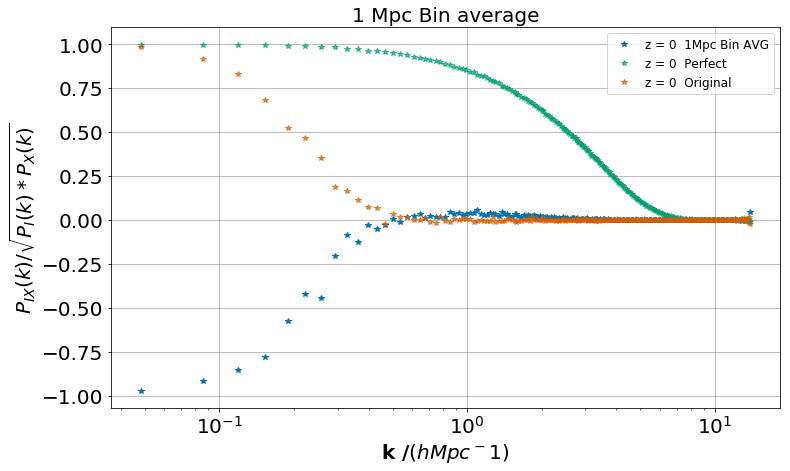
\includegraphics[width=1\columnwidth]{images/realRecon/1MpcBinAvg.png}%
    
    \caption{
        Simulation A reconstruction
        }
        
        \label{fig:last}
\end{figure}

\section{Future Work}
    
There were many interesting results discovered during this project. Perhaps the best example is the almost perfect anti-correlation obtained in some cases. Figure~\ref{fig:last} shows one of the most extreme cases. To perform this reconstruction, we averaged velocities over 1 Mpc bins, interpolated the velocities back onto the particles and then applied the Zel'dovich offset as described in Chapter 3. The resulting correlation is almost a (negative) mirror image of the original correlation. We saw in Section 3.1.3 that the Zel'dovich reconstruction leads to some anti-correlation on the largest scales when starting at low redshifts. This could be explained by the fact that most particles are past shell crossing at this stage. Also, high density collapsed regions tend to have higher peculiar velocities. Because we just use these velocities just once to calculate the displacement (we don't re-evaluate it as we go back in time), we are displacing most of the matter in these regions. However, we know that this must have been a large overdensity at early times (in order to have formed a massive filament). This then leaves us with an anti-correlation. On the other hand, a perfect anti-correlation of the largest scales is very hard to explain and should be studied further. 

Another possible extension of this work would be to smooth the density field. When performing the reconstruction we have assumed perfect knowledge of the final density field, which of course is not the case in practice. Therefore, a further step that would increase the realism of this method would be to also smooth the density field in a manner similar to our smoothing of the velocity field.

The perfect reconstruction has achieved vastly better results than any realistic reconstruction we have attempted. This leads us to conclude that there is much space for the improvement of these methods. We have only used the first order approximation to Lagrangian Perturbation Theory. Higher order approximations could perform better, and also solve some of the problems we encountered.
    


\printbibliography{}

\end{document}
